\documentclass[12pt]{article}
\setcounter{section}{-1}
\usepackage{graphicx}

\begin{document}

\title{%
  Fast Trajectory Replanning \\
  \large CS440 - Intro to Artificial Intelligence}

\author{Alexander Rozenblit}


\maketitle

\section{Introduction}
This assignment implements fast trajectory replanning through the use of the A* search algorithm. After creating a grid world of size 101 x 101, each tile is marked as either a blockage, a start state, a goal state, or an unblocked tile. By using repeated forward A* search, we are able to find the shortest path from the start state to the goal state. We will then compare repeated forward A* with backward A* and adaptive A*, as well as testing the efficiency of using G value tie breaking.

\section{Understanding the Methods}
a) Since the agent does not know about all the obstacles in the grid, the agent evaluates its first move as being to either E3, E1, or D2. The agent needs to move to the square with the smallest f value. The formula for f value is $f(s) = g(s) + h(s)$. The g(s) remains constant for each move, because the agent starts out at E2. So, the move that A* will choose will be the state with smallest h value or heuristic. The heuristic for this problem is simply Manhattan Distances, so we can simply compare the h values for E3,E1, and D2. $h(E3) = 2$, $h(E1) = 4$, and $h(D2) = 4$. Since E3 has the smallest Manhattan Distance, therefore the smallest heuristic and f value, the agent would move there.  \\
\\
b)  The agent will either find the target or realize that it is impossible to reach the target in finite time. Since the grid world is finite the A* algorithm will be able to expand and check every state for a path to get to the target. A finite amount of states to check means the algorithm will eventually terminate.\\
\\
The worst case run time scenario for A* is if every cell without an obstacle is added to the open set and expanded. Let $s$ represent the amount of unblocked spots in the grid. The worst case scenario is for the agent to need to move through every single unblocked cell so that would take $s$ steps. Technically each state expansion might need to make those $s$ steps. So if $s$ states need to go through all $s$ spots that would take $s^{2}$ moves to either get to the target or discover that no such path exists. This is the worst case scenario, and usually the A* search algorithm has a significantly better run time.\\

\section{The Effects of Ties}

One of the ways to optimize an A* search is by the use of G value tie breaking. If the F values of multiple states were equal, then the algorithm would resort to expanding either the state with the lowest or highest G value. To test which tie breaker is more efficient a timeAnalysis.py file was created to run the algorithms while timing them and counting the number of expansions. \\
\\
The higher G score tie breaking strategy proved faster and more efficient than the lower G score tie breaking strategy. Looking at multiple sets of grids after the A* algorithm it is evident that by using the state with a higher G score in a tied scenario, significantly less states are explored. Less states being expanded should theoretically mean a faster completion time, and that is exactly the results the testing yielded. After the test on repeated forward A* with a higher G score as a tie breaker and a repeated forward A* with a lower G score as a tie breaker, it is clear the the higher G score strategy is faster. Below are the times it took for both tests.  To run the test the same 200 grids were solved by both algorithms, and the respective times were divided by 200 to give the time per grid. The same was done with the number of expanded states. The results are below:\\


\begin{center}
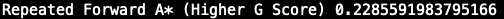
\includegraphics{higherGScore.png}
\end{center}

\begin{center}
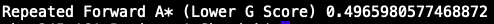
\includegraphics{lowerGScore.png}
\end{center}

\begin{center}
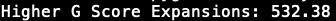
\includegraphics{higherGScoreExp.png}
\end{center}

\begin{center}
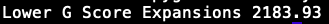
\includegraphics{lowerGScoreExp.png}
\end{center}
This results makes sense, because the higher the G score of the state the further it is from the start state. A majority of the time this means that since it is further from the start state it is closer to the goal state, therefore being the optimal move.\\

\section{Forward vs Backward}

Repeated forward A* and repeated backward A* work very similarly, with the key difference being that forward starts searching from the agent and ends once the target is reached, while backward starts from the target and searches for the agent. After running multiple tests and inspecting multiple grids it is seen that the amount of cells expanded by both the forward and backward search is very similar. In some cases the forward explored a few more cells and in other cases the backward explored more. To test further I timed both tests. Similar to the previous test, 200 of the same grids were solved using both forward and backward repeated A* search. The total time was divided by 200 to give the time per grid. The same was done for cells expanded. The results are below:\\

\begin{center}
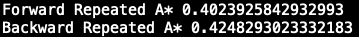
\includegraphics{forwardBackward.png}
\end{center}

\begin{center}
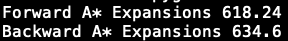
\includegraphics{forwardBackwardExp.png}
\end{center}
These results support what is expected, because there is no advantage in starting from the agent or the target. Even though on some grids forward was faster and others backward was faster, on average both algorithms performed similarly. It does not matter whether the path is solved from the agent or target, because the heuristic and tie breaking procedure remains the same. The minor differences in specific grids can be blamed on the obstacles of that specific grid. Certain configurations of obstacles make it more difficult to find the correct path initially, but both the forward A* and backward A* algorithms struggle with this problem equally.\\

\section{Heuristics in the Adaptive A*}

A heuristic is said to be consistent if its estimate is always less than or equal to the estimated distance from any neighboring state to the goal, plus the cost of reaching that neighbor.  Since the agent can only move four different directions, the cost from the current node to the successor node will always be 1. $1 + h(successor) \geq h(current)$. If the agent moves a step closer to the target the heuristic from the new cell is exactly equal to the old heuristic plus one. While if the agent does any move that does not bring it closer to the target the new heuristic plus one will definitely be greater than the old heuristic, because the agent is now further from the target. By using Manhattan Distances as the heuristic the estimate is accurate, because similar to the way the agent moves, Manhattan Distances are never counted diagonally, but can only move North, South, East, and West. \\
\\
Firstly, the first round of adaptive A* search generates the heuristic using Manhattan Distances, and that is consistent for the reason listed above. Once the algorithm begins modifying the heuristics the heuristic stays consistent. The new heuristic is $h(s) = g(Sgoal) - g(s)$. Since this new estimation is the actual amount of moves it took for the agent to reach the target in a previous search, that number is either equal to the Manhattan Distance heuristic, or (in most cases) greater than the original heuristic, because the agent ran into obstacles. Since the adaptive heuristic will never be less than the Manhattan Distance heuristic it will always be consistent. \\

\section{Heuristics in the Adaptive A*}

Another optimization implemented is Adaptive A* search. Forward A* search consistently used Manhattan Distances as its heuristic, while adaptive A* used previous grid searches to make certain cells' heuristics more accurate. The heuristic of cells that were visited in previous searches were modified before the algorithm began, to be exactly the amount of steps it took to get from that state to the target in the previous searches. \\
\\
This optimization was clever, because even though adaptive A* did not decrease the amount of states visited in the first several searches, as the test ran each maze had less and less visited cells. Since the algorithm was "learning" from previous searches each next search visited less cells and was therefore faster. The heuristic improved with every grid making the algorithm more efficient. Towards the end of the grids however, the adaptive A* plateaued in terms of efficiency, because each grid was barely gaining any new heuristic information from the last.  To test whether this indeed made adaptive A* a faster algorithm, I ran a time test. Like the previous tests, forward and adaptive A* both had to search 200 mazes (4 sets of 50 mazes for adaptive). The times were divided by 200 to find the average per grid. The same was done with counting the expanded states per grid. The results are below:\\
\\

\begin{center}
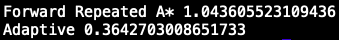
\includegraphics{adaptive.png}
\end{center}

\begin{center}
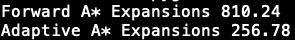
\includegraphics{adaptiveExp.png}
\end{center}
Just as expected the time of adaptive A* search is significantly less than forward repeated A* search. Adaptive A* had more precise and accurate heuristics and therefore was more efficient.

\section{Memory Issues}

It is important to minimize memory usage per each state, because even though the current implementation works for grids of 101X101, problems could be encountered with larger grid sizes, for example 1001X1001.\\
\\
To start, the current implementation creates an 101X101 2D list of states. Each state is an object that contains g value(int), h value(int), f value(int), tree(pointer), and search value(int). \\
\\
$int = 24$ bytes\\
$reference = 8$ bytes\\
$total states = 101 * 101 = 10,201$\\
\\
Memory used in each state  $= 24 * 4 + 8 = 104$  bytes\\
Memory  used in entire grid $= 10,201 * 104 = 1,060,904$ bytes\\
\\
In order to reduce the amount of memory used per grid we can start by understanding not every state needs to be created and stored before the A* search algorithm begins. It is possible to only remember the states that contain obstacles, the agent, and the target. These states can be stored in their own list or dictionary and referenced when needed. As the A* algorithm runs newly visited states are created and stored. Since in almost all searches not every state is expanded this will reduce the amount of states stored per grid.\\
\\
Next, we can optimize the specific attributes that a state object contains. As stated in the assignment the tree pointer can be significantly reduced down to 2 bits. Since there are only 4 places to move from a state the different moves can be mapped to a 2 bit number(North = 00, South = 01, East = 10, West = 11). We can also optimize the specific G, H, and F values. It is possible to only store F values out of those three. The H value can be calculated from inside the search algorithm when it is needed by simply calling the heuristic function. Now since the H value can be computed and the F value is stored it is possible to compute the G value. $f(s) - h(s) = g(s)$.\\
\\
With these optimization in consideration we can recalculate the total memory needed to store a single grid. Since it is impossible to create a constant value for the amount of states expanded per grid I will use the average expanded states over 200 grid iterations (532 states). So the amount of states in each grid will be the obstacles that occur with 0.3 frequency plus the average amount of states expanded. \\
\\
Memory used in each state $= 24*2 + \frac{2}{8} = 48.25$ bytes\\
Total states stored $= 0.3 * (101*101) + 523 = 3,583$ bytes\\
Memory used in the entire grid $=48.25 * 3583 = 172,880$ bytes\\
\\
This optimization reduces memory used by 83.70\%\\
\\
Applying this to a 1001X1001 grid:\\
\\
Total states stored $= 0.3 * (1001*1001) + (\frac{523}{10201} * 1002001) = 351,972$ bytes\\
Memory used in the entire grid $= 351972 * 48.25 = 16,982,649$ bytes\\
\\
The max grid size running on a maximum of 4MB can be represented using this formula.\\
\\
x = length of one side of grid\\
\\
$4*10^{6} = 48.25 * (0.3*x^{2} + (\frac{523}{10201} * x^{2}))$\\
\\
$x = 485$\\
\\
The maximum grid size in a 4MB  max environment with my memory optimizations is 485X485.

\end{document}